\documentclass[10pt]{article}         % the type of document and font size (default 10pt)
\usepackage[margin=1.0in]{geometry}   % sets all margins to 1in, can be changed
\usepackage{moreverb}                 % for verbatimtabinput -- LaTeX environment
\usepackage{url}                      % for \url{} command
\usepackage{amssymb}                  % for many mathematical symbols
\usepackage[pdftex]{lscape}           % for landscaped tables
\usepackage{longtable}                % for tables that break over multiple pages
\usepackage[utf8]{inputenc}           % UTF8 characters
\usepackage[T1]{fontenc}
\usepackage{textcomp}
\usepackage[english]{babel}
\usepackage{float}                    % Position of figure, table
\usepackage{enumitem}                 % Alphabet list
\usepackage{makecell}                 % Customize cells in a table
\usepackage{amsmath}
\usepackage{amsfonts}
\usepackage{amssymb}
\usepackage{mathtools}
\usepackage{graphicx}
\usepackage{babel,blindtext}
\graphicspath{ {../output/} }
\DeclarePairedDelimiter{\ceil}{\lceil}{\rceil}
\renewcommand{\baselinestretch}{1.5}
\title{COCS 6323: Statistical Methods in Research \\ Group Project} % to specify title
\author{Group <number> \\
        Department of Computer Science\\
        University of Houston}         % to specify author(s)
\usepackage{Sweave}
\begin{document}                      % document begins here
\Sconcordance{concordance:ProjectReport.tex:ProjectReport.Rnw:%
1 31 1 1 0 13 1}
\Sconcordance{concordance:ProjectReport.tex:././sections/contribution2.Rnw:ofs 46:%
1 11 1}
\Sconcordance{concordance:ProjectReport.tex:ProjectReport.Rnw:ofs 58:%
47 2 1}
\Sconcordance{concordance:ProjectReport.tex:././sections/section4.Rnw:ofs 61:%
1 9 1}
\Sconcordance{concordance:ProjectReport.tex:ProjectReport.Rnw:ofs 71:%
51 2 1}
\Sconcordance{concordance:ProjectReport.tex:././sections/sectionT2.Rnw:ofs 74:%
1 32 1}
\Sconcordance{concordance:ProjectReport.tex:ProjectReport.Rnw:ofs 107:%
55 2 1}
\Sconcordance{concordance:ProjectReport.tex:././sections/sectionT3.Rnw:ofs 110:%
1 65 1}
\Sconcordance{concordance:ProjectReport.tex:ProjectReport.Rnw:ofs 176:%
59 4 1}


\setkeys{Gin}{width=1.0\textwidth}

\maketitle              % makes the title

\newpage
\tableofcontents        % inserts TOC (section, sub-section, etc numbers and titles)
\listoftables           % inserts LOT (numbers and captions)
\listoffigures          % inserts LOF (numbers and captions)

\newpage
\section{Figure 2A}
% !Rnw root = ../ProjectReport.Rnw
Giant Component\\
\begin{figure}[!htb]
  \minipage{0.32\textwidth}
    \textbf{1990}\\
    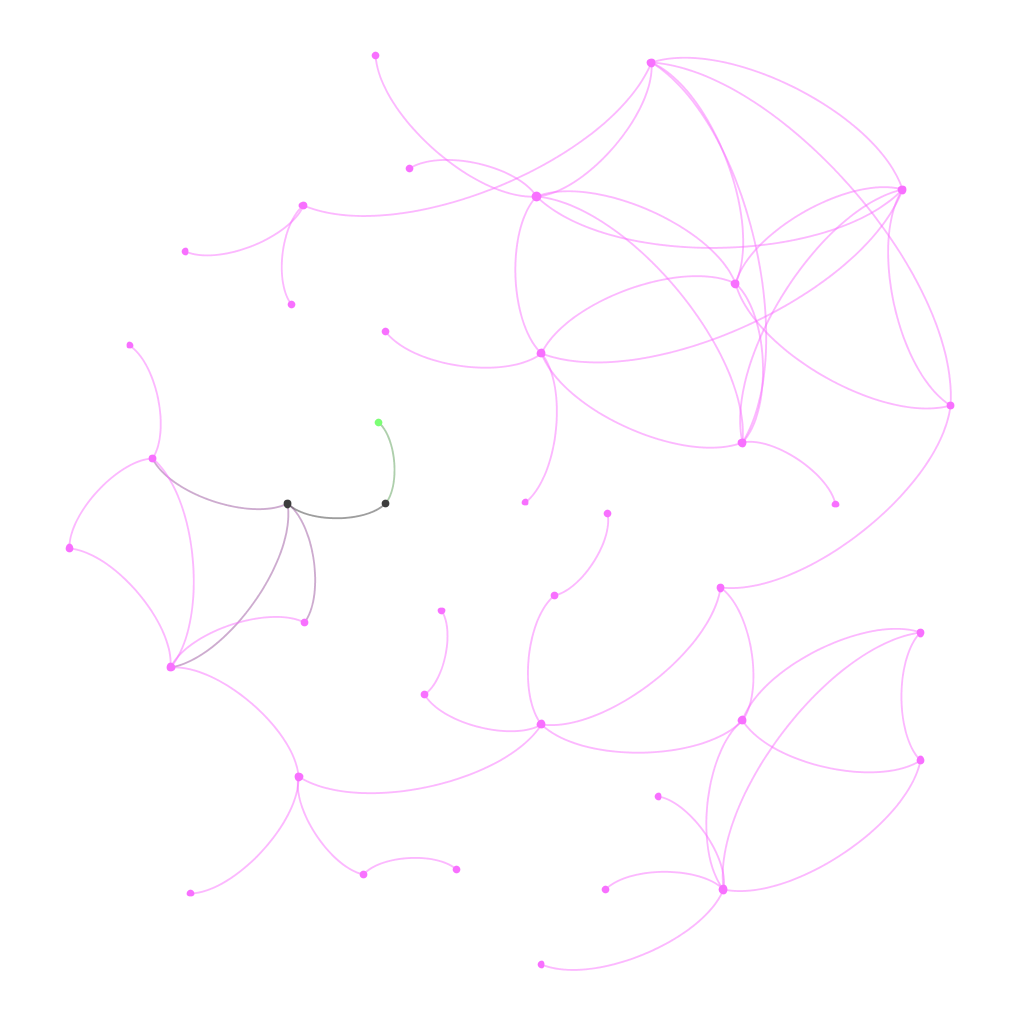
\includegraphics[width=5cm, height=5cm]{Fig2A1990.png}
  \endminipage\hfill
  \minipage{0.32\textwidth}
    \textbf{1995}\\
    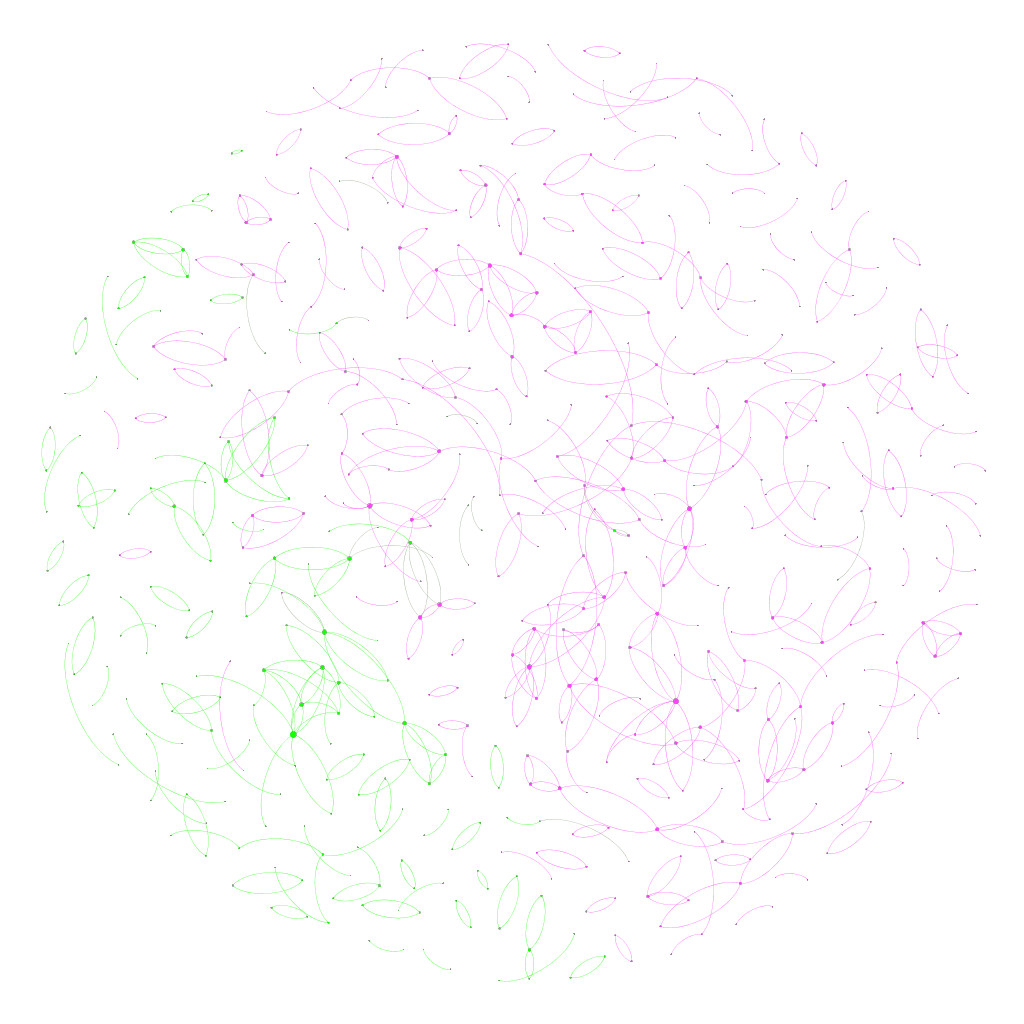
\includegraphics[width=5cm, height=5cm]{Fig2A1995.png}
  \endminipage\hfill
  \minipage{0.32\textwidth}%
    \textbf{2000}\\
    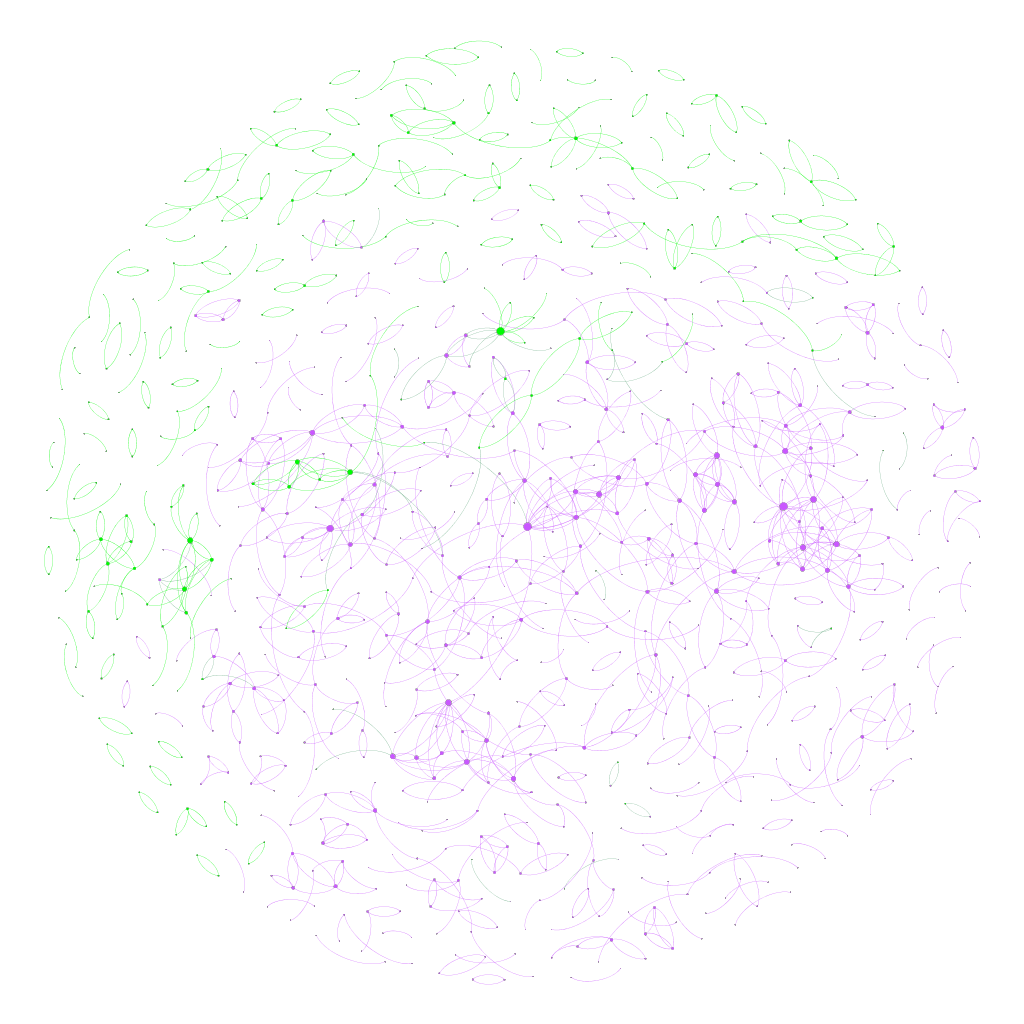
\includegraphics[width=5cm, height=5cm]{Fig2A2000.png}
  \endminipage\hfill
  \minipage{0.32\textwidth}
    \textbf{2005}\\
    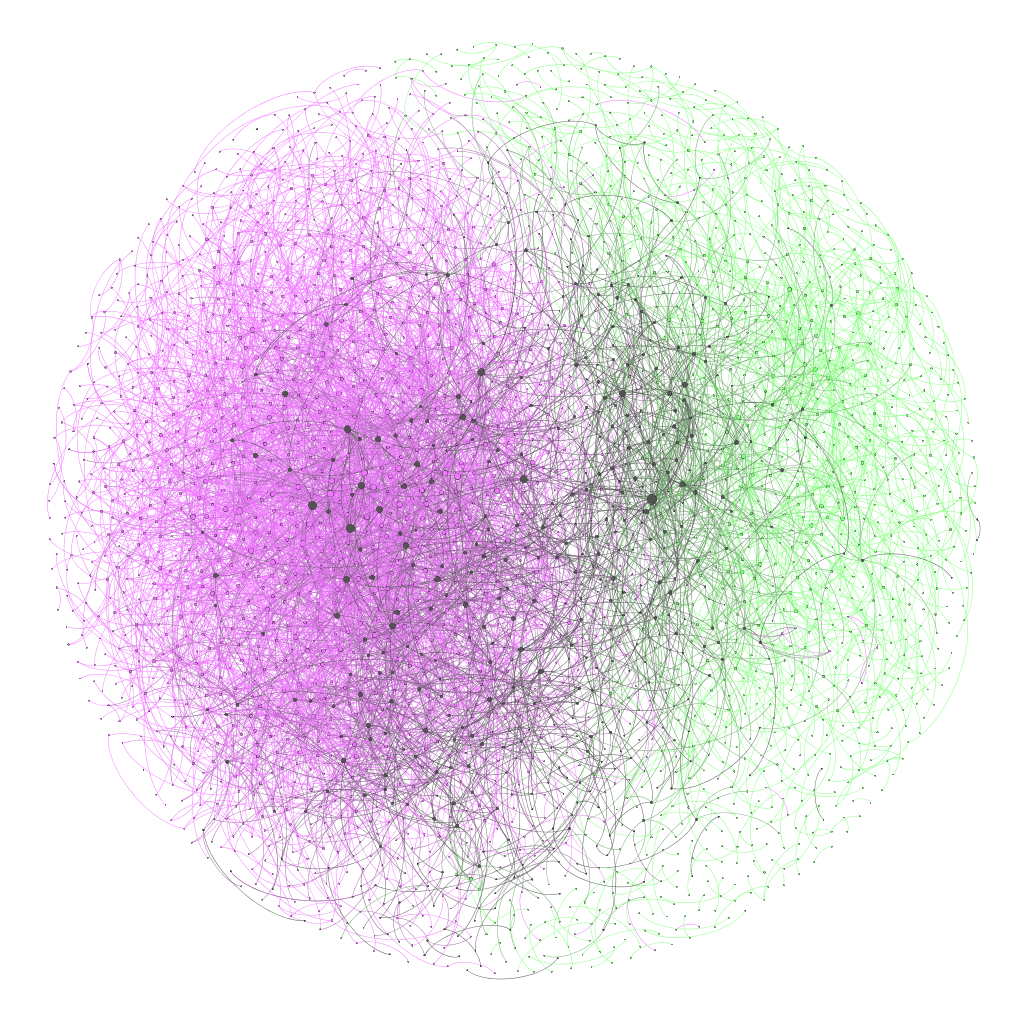
\includegraphics[width=5cm, height=5cm]{Fig2A2005.png}
  \endminipage\hfill
  \minipage{0.32\textwidth}
    \textbf{2010}\\
    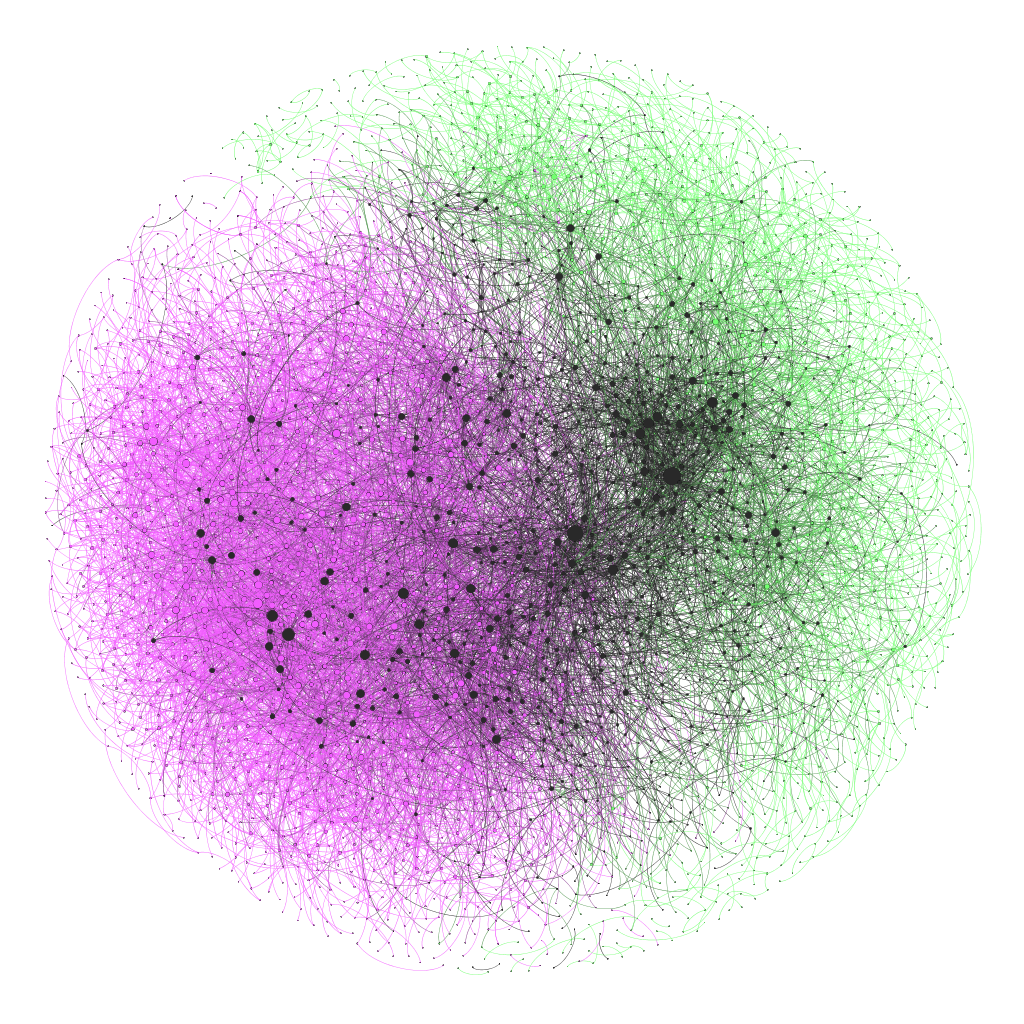
\includegraphics[width=5cm, height=5cm]{Fig2A2010.png}
  \endminipage\hfill
  \minipage{0.32\textwidth}%
    \textbf{2015}\\
    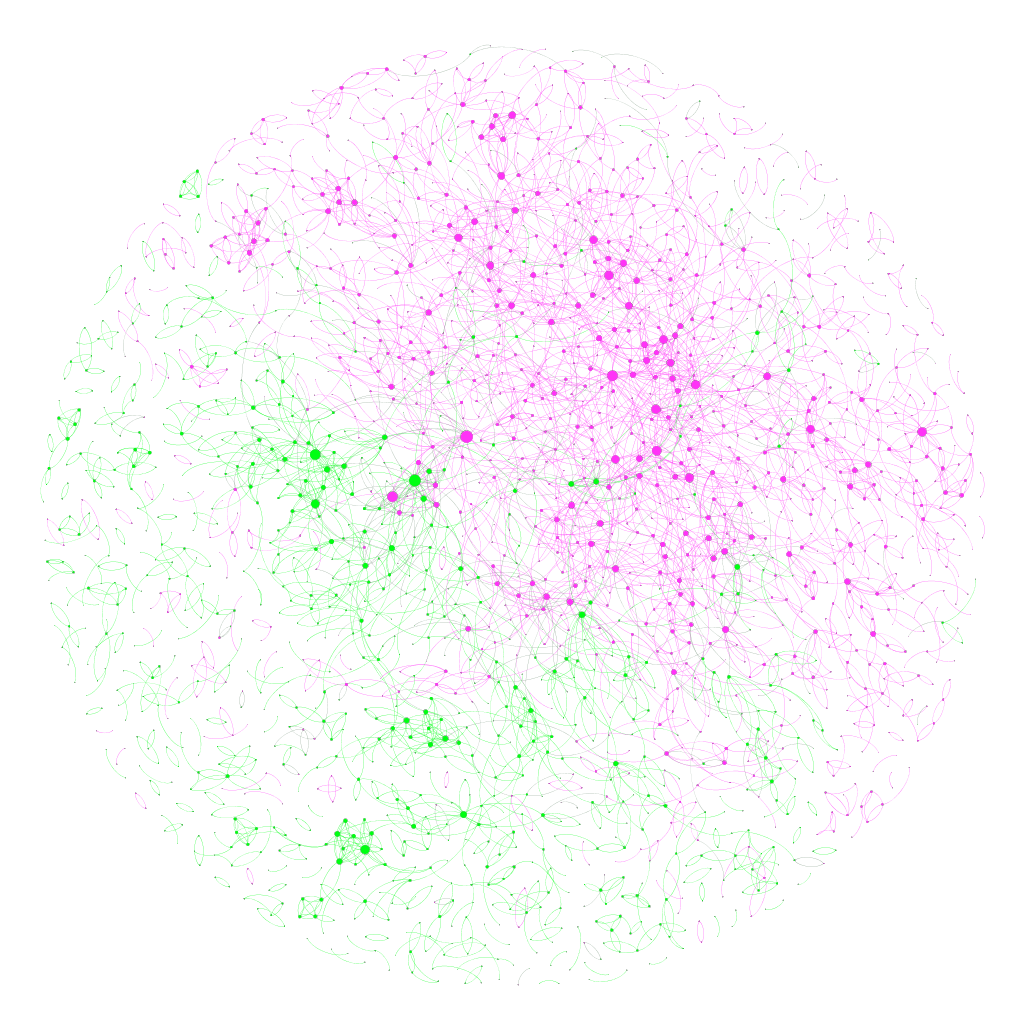
\includegraphics[width=5cm, height=5cm]{Fig2A2015.png}
  \endminipage
  \caption{Growth of cross-disciplinary social capital}
  \label{fig:2A}
\end{figure}\\
Evolution of the giant component in the U.S. biology-computing network. Green and magenta nodes rep- resent faculty F i with BIOF and CSF affiliation, respectively; black nodes represent faculty F i that, by time t, published at least one cross-disciplinary publication and joined the XDF group; node size is proportional to the logarithm of the degree centrality, ln C Di , of F i at time t.

\newpage
\section{Figure 2B}
% !Rnw root = ../ProjectReport.Rnw
\begin{figure}[!htb]
  \centering
  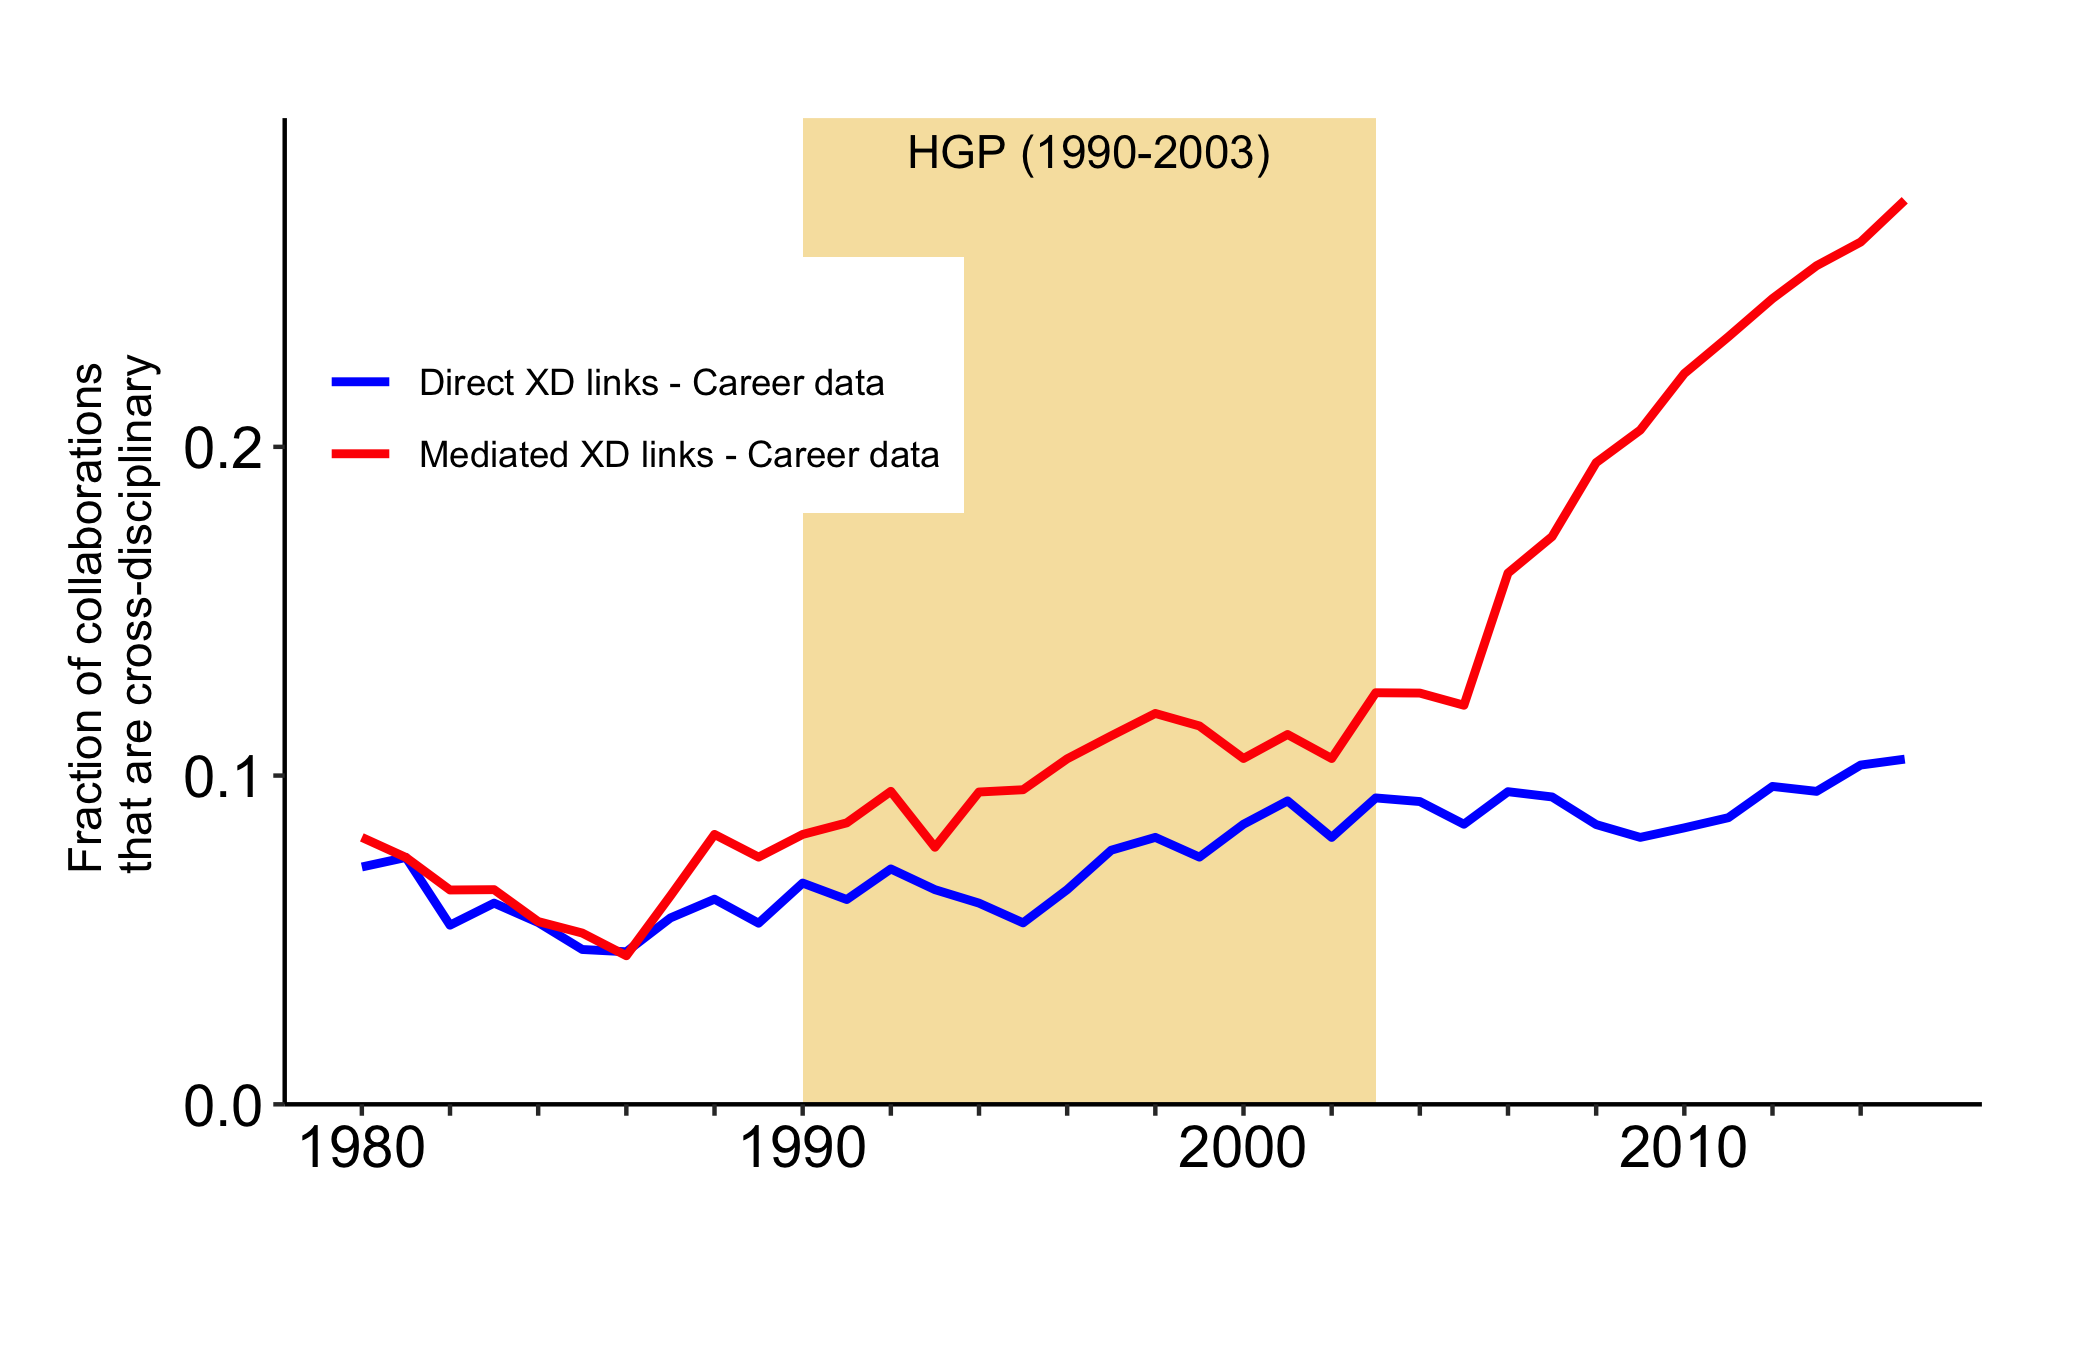
\includegraphics[width=10cm, height=7cm]{Fig2B.png}
  \caption{Growth of cross-disciplinary social capital}
  \label{fig:2B}
\end{figure}

\newpage
\section{Figure 3A}
% !Rnw root = ../ProjectReport.Rnw
Add the content of this section

\newpage
\section{Figure 3B}
% !Rnw root = ../ProjectReport.Rnw
Add the content of this section

\newpage
\section{Figure 3C}
% !Rnw root = ../ProjectReport.Rnw
Add the content of this section

\newpage
\section{Figure 3D}
% !Rnw root = ../ProjectReport.Rnw
Add the content of this section

\newpage
\section{Figure 3E}
% !Rnw root = ../ProjectReport.Rnw
Add the content of this section

\newpage
\section{Figure 3F}
% !Rnw root = ../ProjectReport.Rnw
Add the content of this section

\newpage
\section{Supplementary S3}
% !Rnw root = ../ProjectReport.Rnw
Centrality\\
\begin{figure}[!htb]
  \minipage{0.32\textwidth}
    \textbf{Degree}\\
    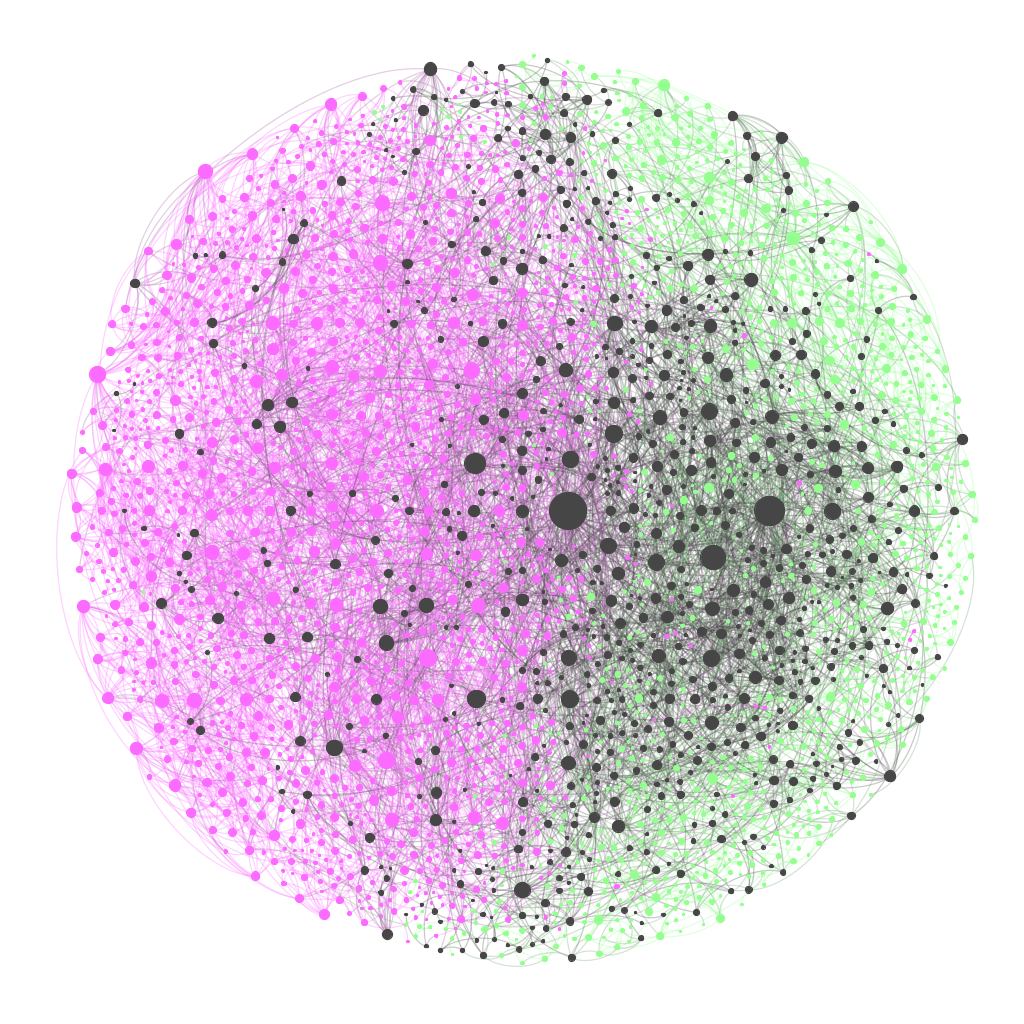
\includegraphics[width=5cm, height=5cm]{S3Degree.png}
  \endminipage\hfill
  \minipage{0.32\textwidth}
    \textbf{PageRank}\\
    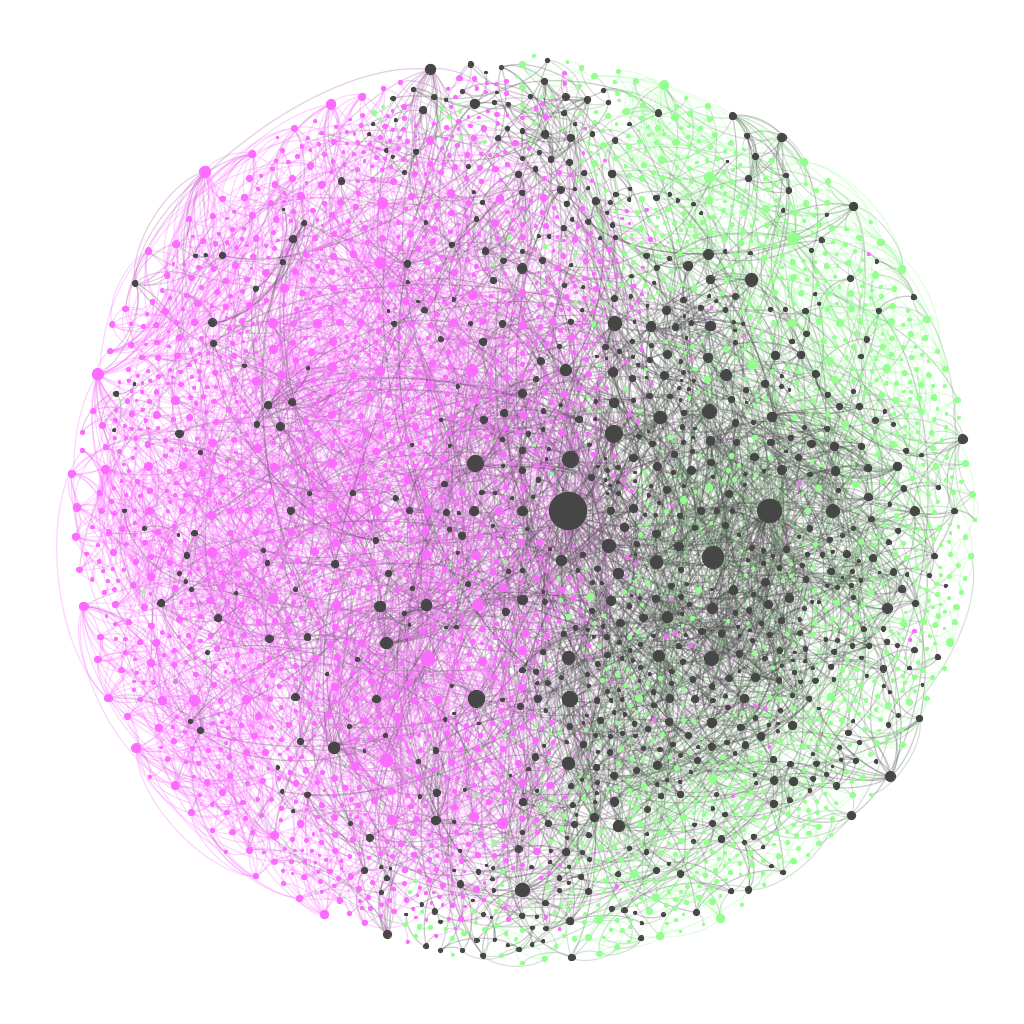
\includegraphics[width=5cm, height=5cm]{S3PageRank.png}
  \endminipage\hfill
  \minipage{0.32\textwidth}%
    \textbf{Betweeness}\\
    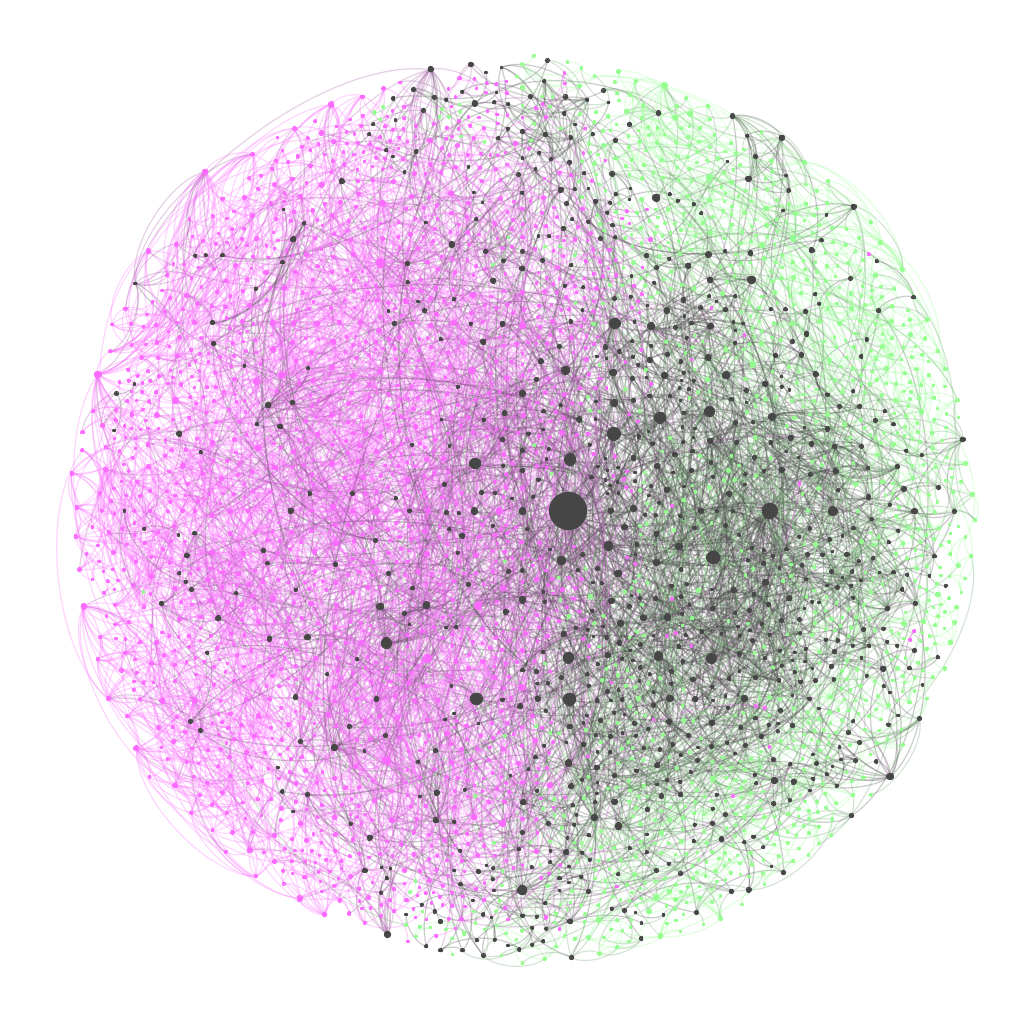
\includegraphics[width=5cm, height=5cm]{S3Betweeness.png}
  \endminipage
  \caption{Three perspectives on the centrality of Fi in the direct collaboration network}
  \label{fig:s3}
\end{figure}

Shown is the giant connected component of the faculty network F using all data up to 2015. The nodes and links across each network are fixed, only the node sizes vary according to the indicated centrality measure:. Notably, the most central according to each of the three measures is Eric Lander, one of the leaders of the HGP.

\newpage
\section{Supplementary S4}
% !Rnw root = ../ProjectReport.Rnw
Dismishing of Giant Component\\
\begin{figure}[!htb]
  \minipage{0.32\textwidth}
    \textbf{1990}\\
    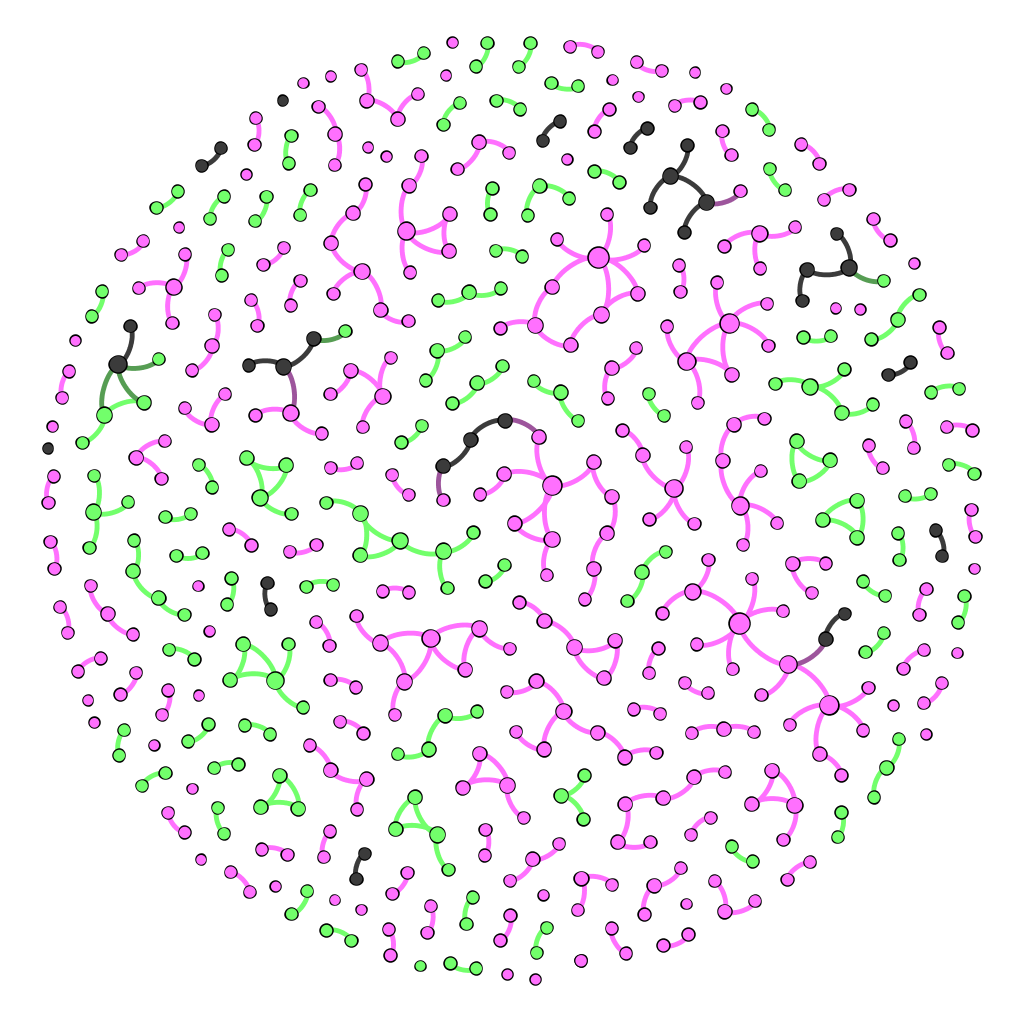
\includegraphics[width=5cm, height=5cm]{S41990.png}
  \endminipage\hfill
  \minipage{0.32\textwidth}
    \textbf{1995}\\
    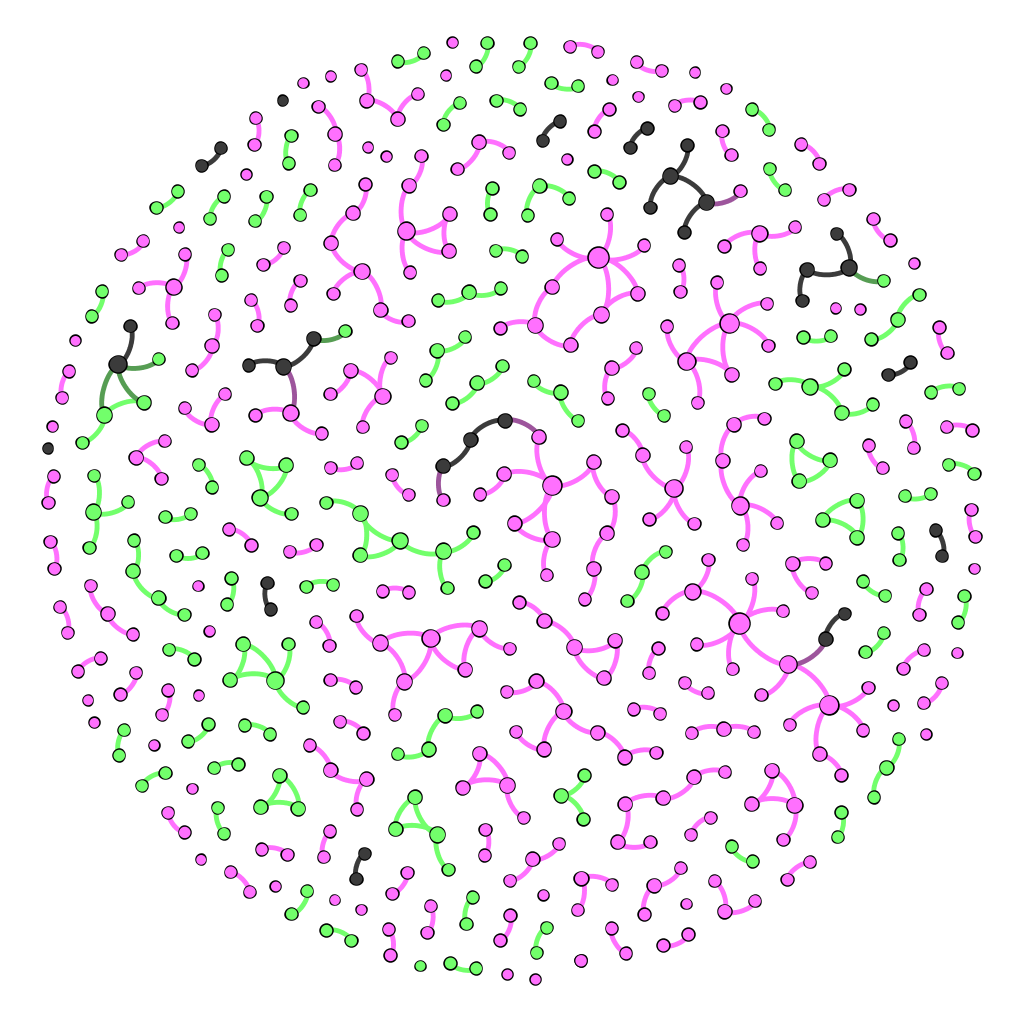
\includegraphics[width=5cm, height=5cm]{S41995.png}
  \endminipage\hfill
  \minipage{0.32\textwidth}%
    \textbf{2000}\\
    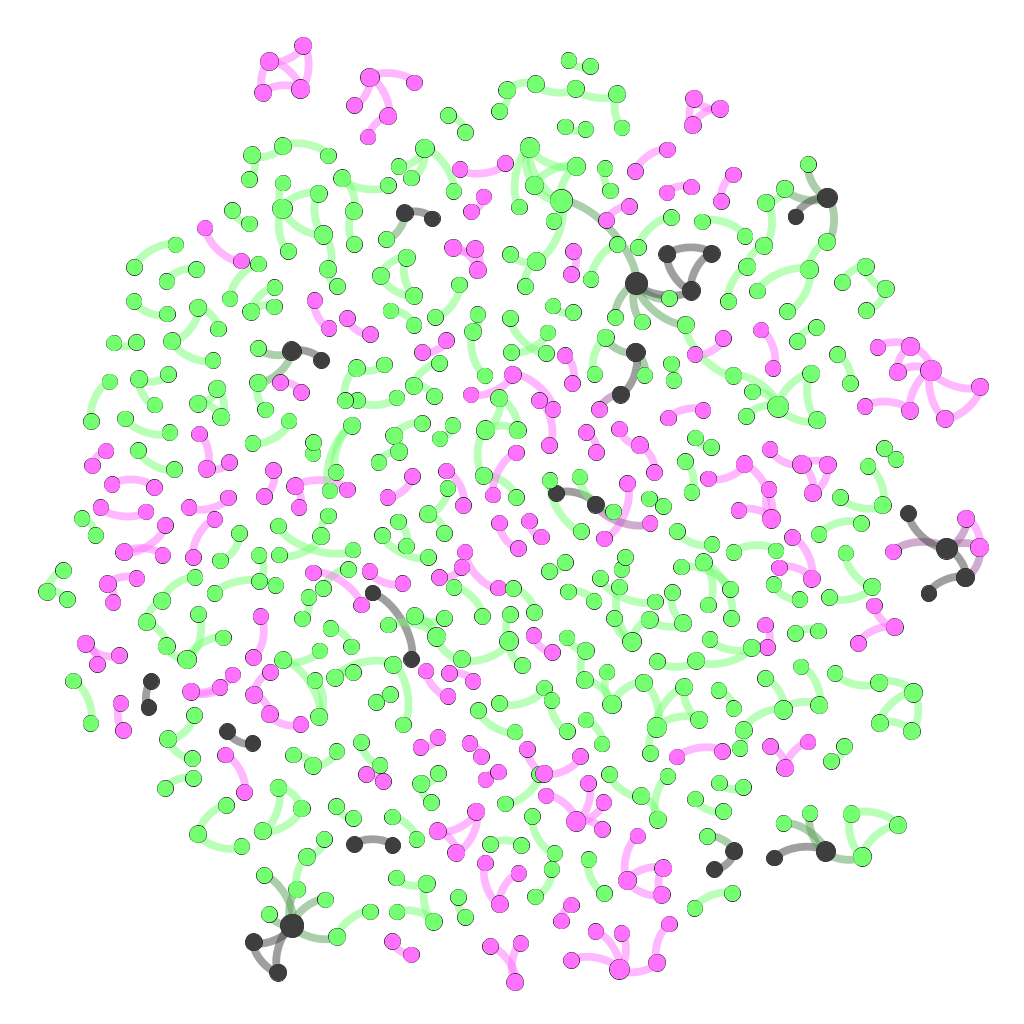
\includegraphics[width=5cm, height=5cm]{S42000.png}
  \endminipage\hfill
  \minipage{0.32\textwidth}
    \textbf{2005}\\
    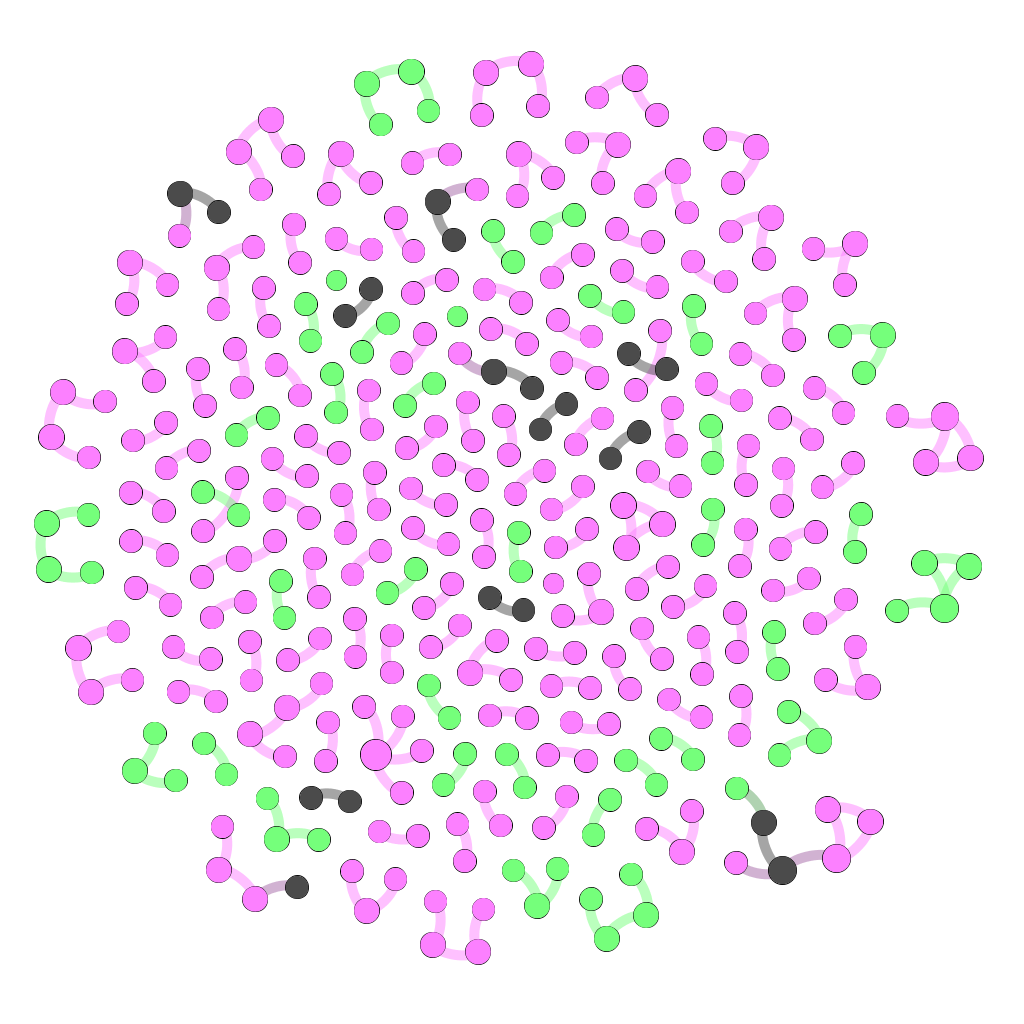
\includegraphics[width=5cm, height=5cm]{S42005.png}
  \endminipage\hfill
  \minipage{0.32\textwidth}
    \textbf{2010}\\
    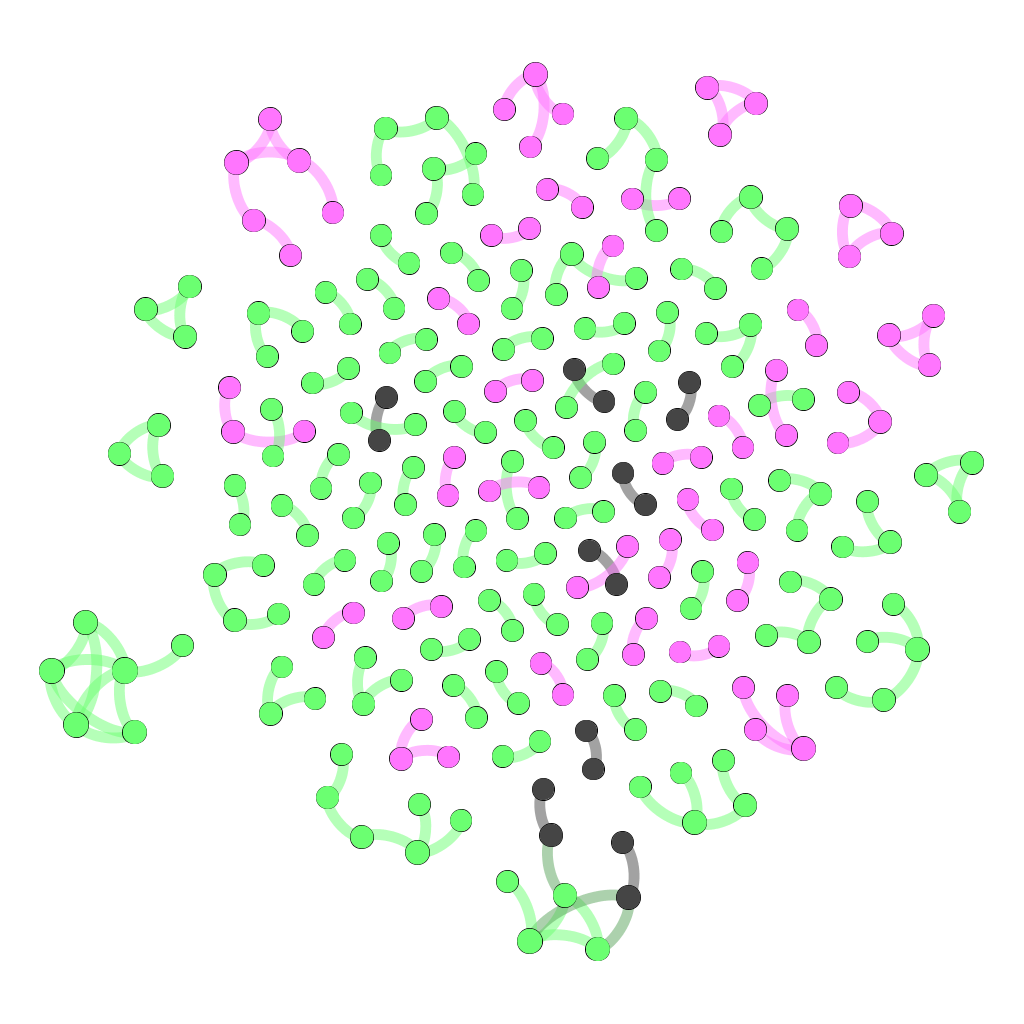
\includegraphics[width=5cm, height=5cm]{S42010.png}
  \endminipage\hfill
  \minipage{0.32\textwidth}%
    \textbf{2015}\\
    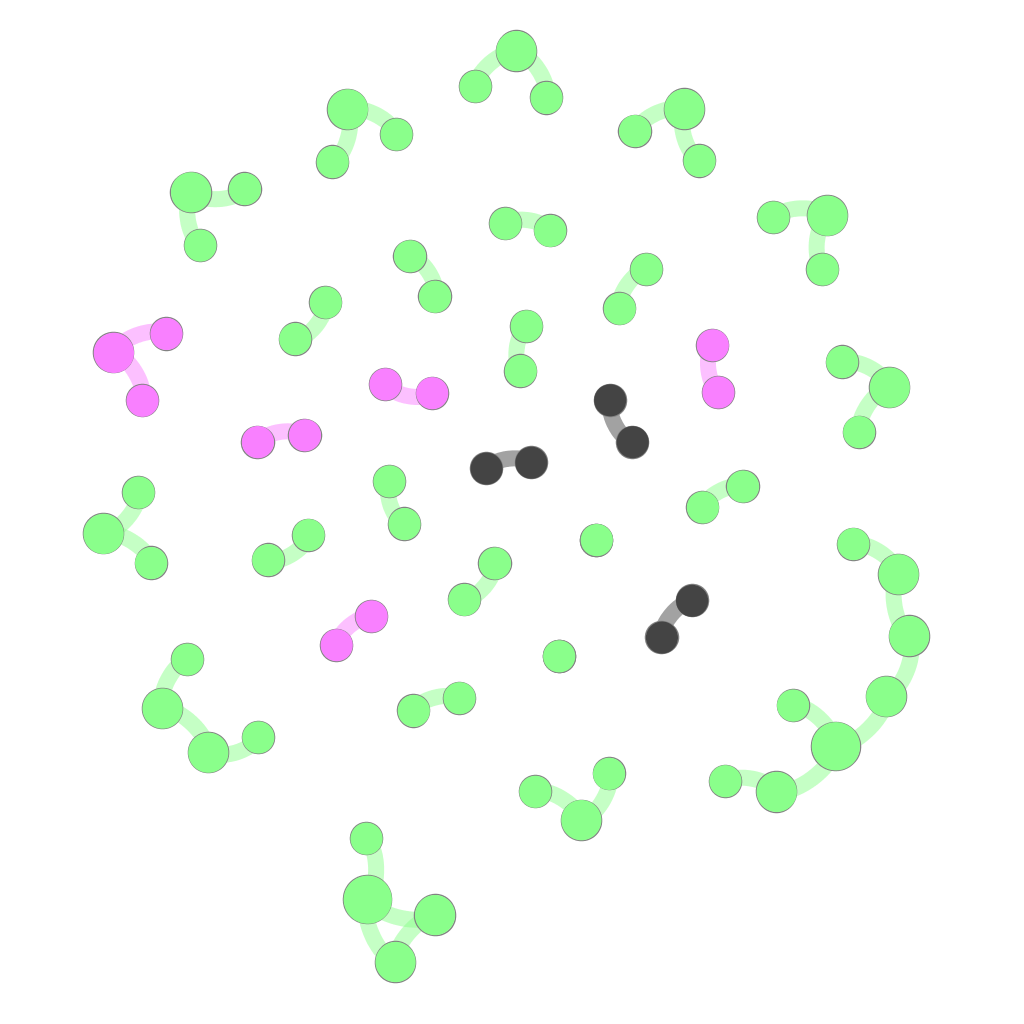
\includegraphics[width=5cm, height=5cm]{S42015.png}
  \endminipage
  \caption{Growth of cross-disciplinary social capital}
  \label{fig:s4}
\end{figure}\\
Green and magenta nodes represent faculty Fi with BIO and CS affiliation, respectively; black nodes represent faculty Fi that by time t collaborated with at least one faculty from the opposite department and thus joined the XD group.


\bigskip   % leave some empty space (optional)

\end{document}

